\chapter{\label{ch:least squares solutions}Least Squares Solutions}

Bolstered from producing concrete results, attention now turns to an examination of solution methods through the lens of the \ft.

\section{\label{sec:ftola}Fundamental Theorem of Linear Algebra}  %    S    S    S    S    S    S    S    S    S    S    S    S  
\index{Fundamental Theorem of Linear Algebra!orthogonal decomposition}
\begin{table}[htbp]  %  T A B L E
    \caption[The Fundamental Theorem of Linear Algebra]{The Fundamental Theorem of Linear Algebra for $\aicmn$ }
    \begin{center}
    		\begin{tabular}{rlcccccccc}
    		  %
    		  domain:   & $\cmplx{n}$ & = & $\brnga{*}$ & $\oplus$ & $\rnlla{}$ \\
    		  %
    		  codomain: & $\cmplx{m}$ & = & $\brnga{}$  & $\oplus$ & $\rnlla{*}$
    		  %
      \end{tabular}
    \end{center}
  \label{tab:ftola}
  \end{table}%

\begin{landscape}
  \begin{table}[ht]
    \caption[The Fundamental Theorem of Linear Algebra in pictures]{The Fundamental Theorem of Linear Algebra and Least Squares for $\aicmn$}
    \begin{center}
      \begin{tabular}{crclc}
          %
          Domain &&&& Codomain \\\hline
          %
          \ \\
          %
          $\cmplxn$ && Mapping && $\cmplxm$ \\[10pt]
          %
          \multirow{3}{*}{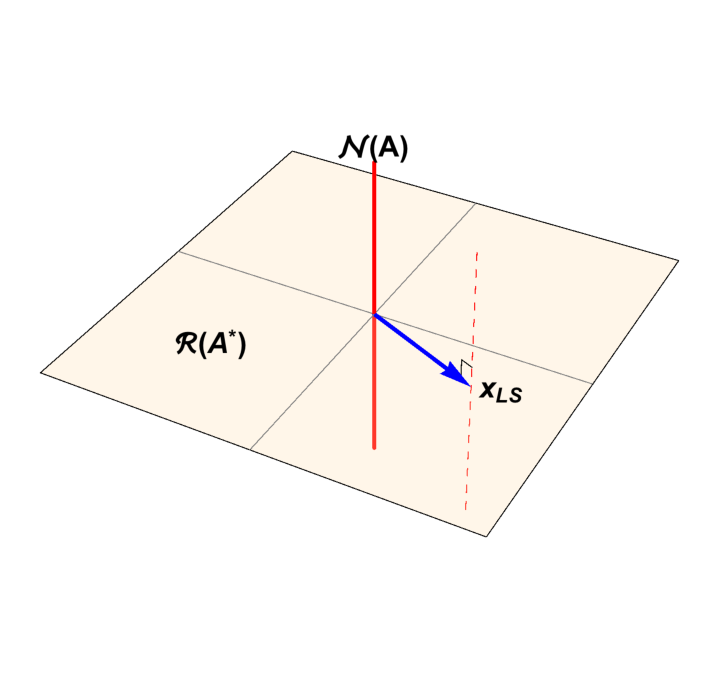
\includegraphics[ width = 2.75in ]{../pdf/theory/ftola/domain}} &&&&
          \multirow{3}{*}{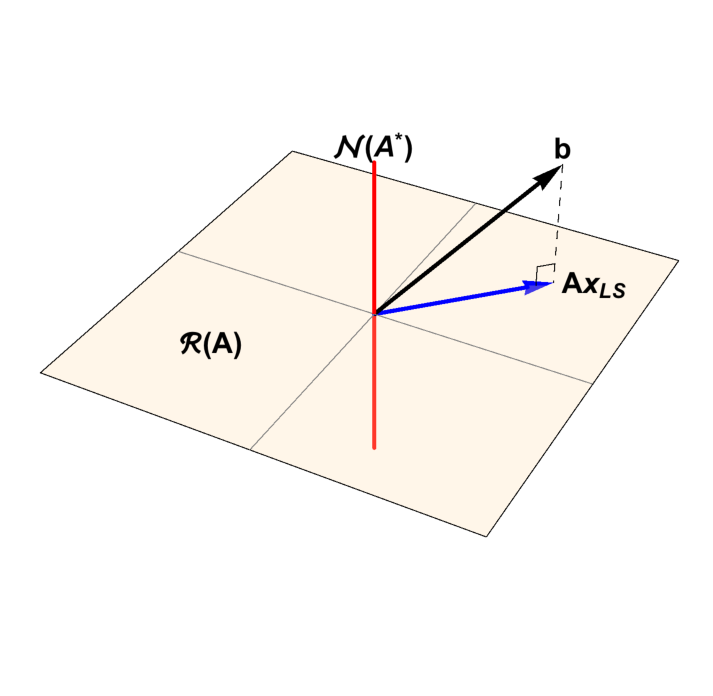
\includegraphics[ width = 2.75in ]{../pdf/theory/ftola/codomain}} \\[55pt]
            & $\A{} \colon \cmplx{n}$ & $\mapsto$ & $\cmplx{m} $ \\[15pt] 
            & $\cmplx{n}$ & $\mapsfrom$ & $\cmplx{m} \colon \A{*}$ \\[80pt]
          %
            $\brnga{*} \oplus \rnlla{}$ &&  && $\brnga{} \oplus \rnlla{*}$
          %
      \end{tabular}
    \end{center}
  \end{table}
\end{landscape}

  \begin{table}[htbp]  %  T A B L E
    \caption{Dimensions of the fundamental subspaces for $\aicmnr$.}
    \begin{center}
      \begin{tabular}{rclcrcl}
        %
        $\dim \paren{\brnga{}}$ & = & $\rho$ && $\dim \paren{\rnlla{*}}$ & = & $m - \rho$ \\
        %
        $\dim \paren{\brnga{*}}$ & = & $\rho$ && $\dim \paren{\rnlla{}}$ & = & $n - \rho$ 
        %
      \end{tabular}
    \end{center}
  %\label{tab:?}
  \end{table}%


\section{\bsvd\ - I}  %    S    S    S    S    S    S    S    S    S    S    S    S
The Fundamental Theorem describes the world as an orthogonal decomposition of the domain and codomain. Why not ask for an orthonormal decomposition? This is precisely what we get from the \asvd.

\subsection{SVD Theorem}  %   SS   SS   SS   SS   SS   SS   SS   SS   SS   SS   SS   SS
Given a matrix $\aicmnr$, a matrix with complex entries with $m$ rows, $n$ columns, and matrix rank $0<\rho\le\min\paren{m,n}$, then there exists a decomposition of the form
  \begin{equation*}   %  =   =   =   =   =
  %\begin{split}
    \svdk{*}
    %\label{eq:}
  %\end{split}
  \end{equation*}
where
\begin{enumerate}
  \item column vectors of unitary matrix $\V{}\icnn$ represent an orthonormal span of the domain,
  \item column vectors of unitary matrix $\U{}\icmm$ represent an orthonormal span of the codomain,
  \item Diagonal entries of $\sig{}\irmn$ contain the singular values; the ordered, nonzero eigenvalues of the product matrix $\wx{*}$.
\end{enumerate}

In block form
  \begin{equation*}   %  =   =   =   =   =
  %\begin{split}
    \A{} = \svd{*} = \csvdblockb{*}
    \label{eq:svd block}
  %\end{split}
  \end{equation*}
Column vectors span the subspaces:
  \begin{equation*}   %  =   =   =   =   =
  \begin{split}
    \V{} &= \vcols,	\\
    \U{} &= \ucols.
    %\label{eq:}
  \end{split}
  \end{equation*}
  \begin{equation*}   %  =   =   =   =   =
  \begin{split}
    \U{} & \icmm , \\
    \V{} & \icnn , \\
    \sig{} & \irmn.
    %\label{eq:}
  \end{split}
  \end{equation*}
  \begin{table}[htbp]  %  T A B L E
    \caption{Orthonormal spans for the invariant subspaces.}
    \begin{center}
      \begin{tabular}{cclcccl}
        %
        && domain &&&& codomain \\\hline
        %
        $\brnga{*}$ &=& span$\lst{\bvo, \dots, \bvrho}$ & \qquad &
        $\brnga{}$  &=& span$\lst{\buo, \dots, \burho}$ \\
        %
        $\rnlla{}$  &=& span$\lst{\rvrpo, \dots, \rvnn}$ &&
        $\rnlla{*}$ &=& span$\lst{\rurpo, \dots, \rum}$ \\
        %
      \end{tabular}
    \end{center}
  %\label{tab:?}
  \end{table}%
  
  \begin{equation*}   %  =   =   =   =   =
  \begin{split}
    u_{j} \cdot u_{k} &= \delta_{jk}, \\
    v_{j} \cdot v_{k} &= \delta_{jk}.
    %\label{eq:}
  \end{split}
  \end{equation*}

Decomposition for \eqref{eq:zonalls}:
  \begin{equation*}   %  =   =   =   =   =
  \begin{split}
    \A{} \phantom{mmmn} &=  \phantom{mmmmn} \U{}  \phantom{mmmnmm} \sig{} \phantom{mmmmmmmmm} \V{*} \\
    \mat{rrc}{-1 & 1 & 0 \\ 0 & -1 & 1} &= 
    \frac{1}{\sqrt{2}} \mat{rc}{\bmo & \bone \\ \bone & \bone }
    \mat{cc|c}{\sqrt{3} & 0 & 0 \\ 0 & 1 & 0}
    \mat{rrc}{
    \bl{\frac{1}{\sqrt{6}}}  & \bl{-\frac{2}{\sqrt{6}}} & \bl{\frac{1}{\sqrt{6}}} \\
    \bl{-\frac{1}{\sqrt{2}}} & \bl{0 \phantom{.}}       & \bl{\frac{1}{\sqrt{2}}} \\
    \rd{\frac{1}{\sqrt{3}}}  & \rd{\frac{1}{\sqrt{3}}}  & \rd{\frac{1}{\sqrt{3}}}
    }
    %\label{eq:}
  \end{split}
  \end{equation*}

  \begin{equation*}   %  =   =   =   =   =
  %\begin{split}
    \ess{} = \mat{cc}{\sqrt{3} & 0 \\ 0 & 1}
    %\label{eq:}
  %\end{split}
  \end{equation*}

\subsection{SVD and Least Squares}  %   SS   SS   SS   SS   SS   SS   SS   SS   SS   SS   SS   SS
A direct implication of the \asvd \ is the homogeneous solution.

\subsubsection{Unitary transformation}  %  SSS  SSS  SSS  SSS  SSS  SSS  SSS  SSS  SSS  SSS  SSS  SSS
The definition of the least squares problem in \eqref{eq:xlsdef} shows that the target of minimization is the quantity
\begin{equation*}
  \rtr{T} = r^{2} = \bminimum .
\end{equation*}
One minimization strategy invokes a unitary transformation to create a simpler problem:
\begin{equation}
  \begin{split} 
    \bminimum 
      &= \normts{ \U{*} \paren{ \bl{\Ax} - b }  }.
  \end{split} 
\end{equation}
This remarkable insight opens a door to solution. Rearranging the \asvd 
\begin{equation*}
  \U{*} \A{} = \sig{} \, \V{*},
\end{equation*}
and using the block form in \eqref{eq:svd block} leads to
\begin{equation*}
  \begin{split} 
    \bminimum 
       = \normts{ \sig{} \, \V{*} x - \U{*} b }
      &= \normts{ \sbb{} \, \cvblockfs{*} x - \cublockfs{*} b } \\
	    &= \normts{ \mat{c}{ \ess{} \bvr{*} x \\[3pt]\hline\zero  } - \mat{c}{ \bur{*} b \\[3pt]\hline \run{*} b } }.
  \end{split} 
\end{equation*}
The range space components are now untangled from the  \ns \ components.

\subsubsection{Pseudoinverse solution}  %  SSS  SSS  SSS  SSS  SSS  SSS  SSS  SSS  SSS  SSS  SSS  SSS
Using the Pythagorean theorem\index{Pythagorean theorem} to isolate the range and \ns \ components of the total error for the least squares problem
\begin{equation*}
  \bminimum = \underbrace{\normts{ \ess{} \bvr{*} x -\bur{*} b  }}_{\substack{x \text{ dependence}\\\text{under control}}} + \underbrace{\normts{ \run{*} b  }}_{\substack{\text{residual}\\\text{no control}}}
\end{equation*}
There are now two terms; the first depends upon the solution vector $x$, the second does not. We only have control over the first term. To minimize the total error we must drive the first term to zero. Then the total error will be given by the residual error\index{least squares!residual error!\ns\ terms} term.
The error term that is controlled by the solution vector $x$ is this
\begin{equation}
  \ess{} \bvr{*} x - \bur{*} b \rightarrow 0.
\end{equation}
Choosing the vector $x$ which forces this term to zero  leads to the SVD solution\index{least squares!solution!SVD} for the least squares problem:
\begin{equation*}
  \xmp = \bvr{} \ess{-1} \bur{*} b.
  \label{eq:svd soln}
\end{equation*}
This is also the pseudoinverse solution\index{least squares!solution!pseudoinverse}
\begin{equation*}
  \xmp = \bl{\Ap b}
\end{equation*}
where the (thin) pseudoinverse is
\begin{equation*}
  \Ap = \bvr{} \ess{-1} \bur{*}.
  \label{eq:mpptsvd}
\end{equation*}
The error that can be controlled is forced to 0; but this leaves an error which cannot be removed, a residual error defined as
  \begin{equation*}   %  =   =   =   =   =
  %\begin{split}
    r^{2} = \normts{ \run{*} b  } .
    %\label{eq:}
  %\end{split}
  \end{equation*}
The usually silent \ns \ term can be heard as it pronounces the value of the total error.

To recap, the \asvd \ leads immediately to the pseudoinverse solution and residual error.

\subsubsection{In retrospect}  %  SSS  SSS  SSS  SSS  SSS  SSS  SSS  SSS  SSS  SSS  SSS  SSS
Decompose the data vector in range and null space components:
  \begin{equation*}   %  =   =   =   =   =
  %\begin{split}
    b = \bl{b_{\atomrng}} + \rd{b_{\atomnll}}
    %\label{eq:}
  %\end{split}
  \end{equation*}

  \begin{equation*}   %  =   =   =   =   =
  %\begin{split}
    \normts{ \bl{\Ax} - b } = \normts{ \underbrace{\bl{\Ax} - \bl{b_{\atomrng}}}_{\zero} - \rd{b_{\atomnll}} } = \normts{ \rd{b_{\atomnll}} }
    %\label{eq:}
  %\end{split}
  \end{equation*}
Because the vector $\bl{b_{\atomrng}} \in \brnga{}$, there exists a vector $x$ such that $\bl{\Ax} = \bl{b_{\atomrng}}$. Again, the error that cannot be removed is the residual error
  \begin{equation*}   %  =   =   =   =   =
  %\begin{split}
    \normts{ \rd{b_{\atomnll}} }
    %\label{eq:}
  %\end{split}
  \end{equation*}
What we shown is that the vector $x$ which minimizes the least squares error in \eqref{eq:lsmin} is exactly the same vector given by the SVD solution in equation \eqref{eq:svd soln}. Using a unitary transform we were able to convert the general least squares problem into a form amenable to solution using the \asvd.

For the overdetermined case as we have here the usually silent \ns \ term can be heard as it pronounces the value of the total error
\begin{equation}
  r^{2} = \normts{ \run{*} b  } = \paren{ \run{*} b  }^{*} \paren{ \run{*} b  } = b^{*} \paren{ \run{}\run{*} } b 
  \label{eq:r2:a}
\end{equation}

\section{\bsvd\ - II}  %    S    S    S    S    S    S    S    S    S    S    S    S
\subsection{Fundamental Projectors}  %   SS   SS   SS   SS   SS   SS   SS   SS   SS   SS   SS   SS
Given a matrix $\aicmnr$, a matrix with complex entries with $m$ rows, $n$ columns, and matrix rank $0<\rho\le\min\paren{m,n}$, then there exists a 

\begin{table}[htbp]  % + + + + T A B L E
    \caption{Fundamental Projectors}
    \begin{center}
        \begin{tabular}{ccccccc}
            %
            \multicolumn{4}{c}{Range space} & \multicolumn{3}{c}{Null space} \\\hline
            %
            $\pra$  & = & $\bur{*}\bur{}$ && $\pnas$  & = & $\I{m} - \bur{*}\bur{}$\\
            %
            $\pras$ & = & $\bvr{*}\bvr{}$ && $\pna$  & = & $\I{n} - \bvr{*}\bvr{}$\\
            %
        \end{tabular}
    \end{center}
    %\label{default}
\end{table}%

\section{Least Squares Solution - Again}  %    S    S    S    S    S    S    S    S    S    S    S    S  
Let's revisit the canonical linear system in \eqref{eq:axeb} the general solution in \eqref{eq:general soln}:
  \begin{equation*}   %  =   =   =   =   =
   \begin{split}
    x_{LS} 
      &= \bsolnls{b}{y} \\
      &= \bl{\Ap b} + \pras y
   \end{split}
  \label{eq:}
  \end{equation*}
where the arbitrary vector $y\in\cmplxn$.

The projector onto the range space $\brnga{*}$
  \begin{equation*}   %  =   =   =   =   =
   %\begin{split}
      \ApA = \V{}\Sigma^{\sym}\Sigma{}\V{*} = \bvr{} \bvr{*}
   %\end{split}
 %\label{eq:}
  \end{equation*}

\endinput